\begin{pastexam}[label={px:ncku-111-prog-03}]{成大資訊聯招 111 學年度 第 3 題}
（選擇與作圖）

\textbf{[2\%, 3\%]} You are given the red-black tree in the following, where the dark colored nodes are red nodes. We insert the data item "62" into the tree. (i) Which of the followings is true? (ii) Please illustrate its 2-3-4 tree counterpart representation after 62 is inserted.

\begin{center}
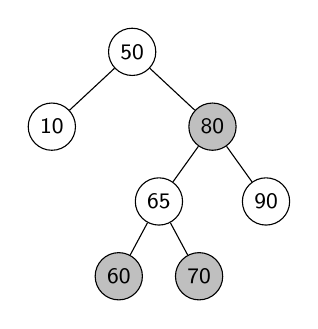
\begin{tikzpicture}[x=0.85cm,y=0.95cm,v/.style={circle,draw,inner sep=0pt,minimum size=6mm,font=\footnotesize\sffamily},s/.style={v,fill=black!25}]
\node[v] (n50) at (1.2,0) {50};
\node[v] (n10) at (0,-1) {10};
\node[s] (n80) at (2.4,-1) {80};
\node[v] (n65) at (1.6,-2) {65};
\node[v] (n90) at (3.2,-2) {90};
\node[s] (n60) at (1,-3) {60};
\node[s] (n70) at (2.2,-3) {70};
\draw (n50)--(n10) (n50)--(n80) (n80)--(n65) (n80)--(n90) (n65)--(n60) (n65)--(n70);
\end{tikzpicture}
\end{center}

(A)
\begin{center}
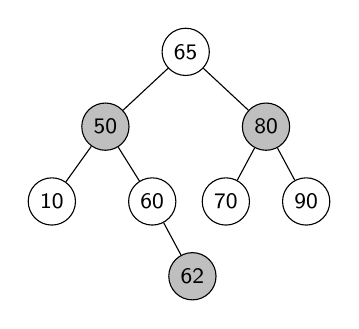
\begin{tikzpicture}[x=0.85cm,y=0.95cm,v/.style={circle,draw,inner sep=0pt,minimum size=6mm,font=\footnotesize\sffamily},s/.style={v,fill=black!25}]
\node[v] (n65) at (2.2,0) {65};
\node[s] (n50) at (1,-1) {50};
\node[s] (n80) at (3.4,-1) {80};
\node[v] (n10) at (0.2,-2) {10};
\node[v] (n60) at (1.7,-2) {60};
\node[v] (n70) at (2.8,-2) {70};
\node[v] (n90) at (4,-2) {90};
\node[s] (n62) at (2.3,-3) {62};
\draw (n65)--(n50) (n65)--(n80) (n50)--(n10) (n50)--(n60) (n80)--(n70) (n80)--(n90) (n60)--(n62);
\end{tikzpicture}
\end{center}

(B)
\begin{center}
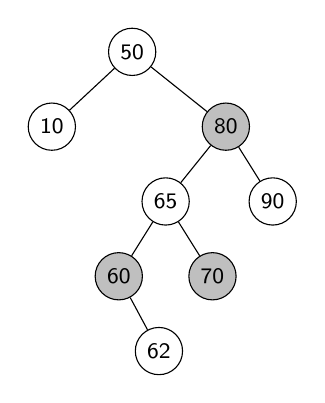
\begin{tikzpicture}[x=0.85cm,y=0.95cm,v/.style={circle,draw,inner sep=0pt,minimum size=6mm,font=\footnotesize\sffamily},s/.style={v,fill=black!25}]
\node[v] (n50) at (1.2,0) {50};
\node[v] (n10) at (0,-1) {10};
\node[s] (n80) at (2.6,-1) {80};
\node[v] (n65) at (1.7,-2) {65};
\node[v] (n90) at (3.3,-2) {90};
\node[s] (n60) at (1,-3) {60};
\node[s] (n70) at (2.4,-3) {70};
\node[v] (n62) at (1.6,-4) {62};
\draw (n50)--(n10) (n50)--(n80) (n80)--(n65) (n80)--(n90) (n65)--(n60) (n65)--(n70) (n60)--(n62);
\end{tikzpicture}
\end{center}

(C)
\begin{center}
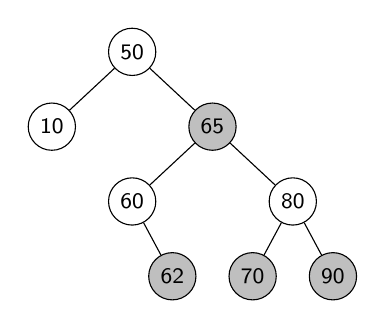
\begin{tikzpicture}[x=0.85cm,y=0.95cm,v/.style={circle,draw,inner sep=0pt,minimum size=6mm,font=\footnotesize\sffamily},s/.style={v,fill=black!25}]
\node[v] (n50) at (1.2,0) {50};
\node[v] (n10) at (0,-1) {10};
\node[s] (n65) at (2.4,-1) {65};
\node[v] (n60) at (1.2,-2) {60};
\node[v] (n80) at (3.6,-2) {80};
\node[s] (n62) at (1.8,-3) {62};
\node[s] (n70) at (3,-3) {70};
\node[s] (n90) at (4.2,-3) {90};
\draw (n50)--(n10) (n50)--(n65) (n65)--(n60) (n65)--(n80) (n60)--(n62) (n80)--(n70) (n80)--(n90);
\end{tikzpicture}
\end{center}

(D)
\begin{center}
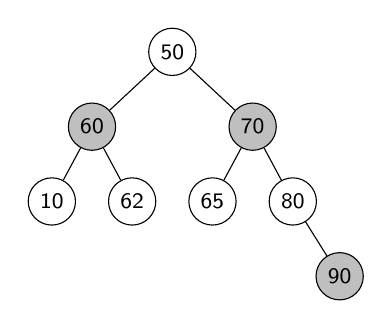
\begin{tikzpicture}[x=0.85cm,y=0.95cm,v/.style={circle,draw,inner sep=0pt,minimum size=6mm,font=\footnotesize\sffamily},s/.style={v,fill=black!25}]
\node[v] (n50) at (2,0) {50};
\node[s] (n60) at (0.8,-1) {60};
\node[s] (n70) at (3.2,-1) {70};
\node[v] (n10) at (0.2,-2) {10};
\node[v] (n62) at (1.4,-2) {62};
\node[v] (n65) at (2.6,-2) {65};
\node[v] (n80) at (3.8,-2) {80};
\node[s] (n90) at (4.5,-3) {90};
\draw (n50)--(n60) (n50)--(n70) (n60)--(n10) (n60)--(n62) (n70)--(n65) (n70)--(n80) (n80)--(n90);
\end{tikzpicture}
\end{center}
\end{pastexam}

\begin{pastsoln}
答案：(i) (A)。 (ii) 2-3-4 樹的根是 $[50, 65, 80]$，四個子節點由左到右是 $[10]$、$[60, 62]$、$[70]$、
$[90]$（圖見最後）。

圖中灰色（深色）的節點是紅色，白色是黑色。 先確認原本的樹：$50$、$10$、$65$、$90$ 黑，$80$、$60$、$70$
紅；從根到每個 NIL 都經過 $2$ 個黑節點，紅節點的子節點都是黑的，是合法的紅黑樹。

\textbf{(i) 插入 $62$}（資結書第~10.3.4~節、虛擬碼~10.6）。
\begin{enumerate}
\item \textbf{當成一般二元搜尋樹插入}：$62 > 50$ 往右到 $80$；$62 < 80$ 往左到 $65$；$62 < 65$ 往左到
$60$；$62 > 60$，成為 $60$ 的右子節點，塗紅色。 這時 $62$ 和父節點 $60$ 都是紅的，要修正。
\item \textbf{$z = 62$}：父節點 $60$ 紅，叔叔 $70$ 也紅，屬於「叔叔是紅色」的情況：$60$、$70$ 改成黑，
祖父 $65$ 改成紅，問題往上移到 $z = 65$。
\item \textbf{$z = 65$}：父節點 $80$ 紅，祖父 $50$，$80$ 是 $50$ 的右子節點，叔叔 $10$ 是黑的。 $65$ 是
$80$ 的左子節點，形成「右、左」的拐彎，先在 $80$ 右旋：$65$ 接到 $50$ 的右邊，$80$ 成為 $65$ 的右子節點，
$65$ 原本的右子樹 $70$ 改接到 $80$ 的左邊。 現在 $z = 80$，父節點 $65$，是一直線的情況。
\item \textbf{一直線的情況}：父節點 $65$ 改黑、祖父 $50$ 改紅，在 $50$ 左旋：$65$ 成為根，$50$ 成為
$65$ 的左子節點，$65$ 原本的左子樹（$60$ 和它的右子節點 $62$）改接到 $50$ 的右邊。 $65$ 是黑的，修正結束。
\end{enumerate}
結果：根 $65$（黑）；$50$（紅）的子節點 $10$（黑）、$60$（黑），$60$ 的右子節點 $62$（紅）；$80$（紅）的
子節點 $70$、$90$（黑）。 這就是 (A)。 檢查：每條根到 NIL 的路徑都經過 $2$ 個黑節點（例如
$65 \to 50 \to 60 \to 62 \to$ NIL 經過 $65$、$60$），沒有紅節點有紅子節點，中序是
$10, 50, 60, 62, 65, 70, 80, 90$。

逐項檢查：
\begin{itemize}
\item (A)：就是上面的結果。 正確。
\item (B)：$62$ 塗成黑色直接掛在 $60$ 下面，沒有做任何修正。 經過 $62$ 的路徑有 $3$ 個黑節點（$50$、
$65$、$62$），其他路徑只有 $2$ 個，違反黑高度相同的性質，而且新插入的節點應該是紅的。 錯。
\item (C)：這棵其實也是合法的紅黑樹（每條路徑 $2$ 個黑節點、沒有連續的紅），但它不是插入演算法得到的
樹：從原樹插入 $62$，修正過程一定會把 $65$ 轉上來當根（第 3、4 步）。 對應的 2-3-4 樹是根 $[50, 65]$、
子節點 $[10]$、$[60, 62]$、$[70, 80, 90]$，和 (ii) 不同。 題目問插入後的樹，錯。
\item (D)：$60$ 是 $50$ 的左子節點，但 $60 > 50$，連二元搜尋樹都不是。 錯。
\end{itemize}

\textbf{(ii) 對應的 2-3-4 樹}（資結書第~10.4~節）：每個黑節點和它的紅子節點合成一個 2-3-4 樹的節點，
黑節點的鍵在中間。
\begin{itemize}
\item 根 $65$（黑）和紅子節點 $50$、$80$：$[50, 65, 80]$，是 4-節點。
\item $10$（黑，沒有紅子節點）：$[10]$；$60$（黑）和紅子節點 $62$：$[60, 62]$；$70$：$[70]$；$90$：$[90]$。
\end{itemize}
\begin{center}
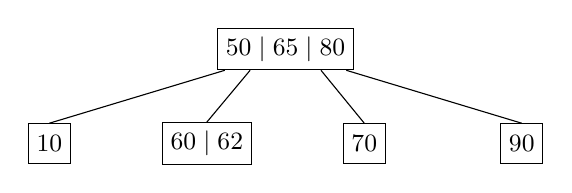
\begin{tikzpicture}[x=1cm,y=1cm,k/.style={draw,rectangle,inner sep=3pt,minimum height=5mm,font=\small}]
\node[k] (r) at (3,0) {$50 \mid 65 \mid 80$};
\node[k] (a) at (0,-1.2) {$10$};
\node[k] (b) at (2,-1.2) {$60 \mid 62$};
\node[k] (c) at (4,-1.2) {$70$};
\node[k] (d) at (6,-1.2) {$90$};
\draw (r.south west)+(0.1,0) -- (a.north);
\draw (r.south)+(-0.45,0) -- (b.north);
\draw (r.south)+(0.45,0) -- (c.north);
\draw (r.south east)+(-0.1,0) -- (d.north);
\end{tikzpicture}
\end{center}
直接在 2-3-4 樹上看也一樣：原樹對應的 2-3-4 樹是根 $[50, 80]$、子節點 $[10]$、$[60, 65, 70]$、$[90]$。
插入 $62$ 要放進 $[60, 65, 70]$，它已經是 4-節點，先分裂：中間的 $65$ 升到父節點，變成 $[50, 65, 80]$，
下面分成 $[60]$ 和 $[70]$；再把 $62$ 放進 $[60]$，得到 $[60, 62]$。 紅黑樹修正的第 2 步（變色）就是這次
分裂，第 3、4 步的旋轉只是把 4-節點 $[50, 65, 80]$ 改成以 $65$ 為黑色中心的畫法。
\end{pastsoln}
